\documentclass[a4paper,12pt]{article}
\usepackage{graphicx, geometry, subfigure, amsmath, adjustbox, array}
\usepackage{xcolor}
\geometry{a4paper,left=2cm,right=2cm,top=1cm,bottom=2cm}
\setlength{\baselineskip}{12pt}
\renewcommand\arraystretch{1.5}
\renewcommand{\d}{\mathrm{d}}
\newcommand{\cm}{\mathrm{cm}}
\newcommand{\s}{\mathrm{s}}
\newcommand{\g}{\mathrm{g}}

\title{\textbf{Stars and Planets Problem Set3}}
\author{Qingru Hu}
\date{\today}

\begin{document}
\maketitle
\section*{\textbf{Exercise \uppercase\expandafter{\romannumeral3}.1  Energetics of collapsing clouds}}
\subsection*{(a)}
The eccentricity, semi-major axis and the orbital period of a particle that starts from $r=R$ and 
collapses towards the center is relatively $e=1$, $a=R/2$ and $T=2t_{\text{ff}}$. From the Kelper 
third law we have:
\begin{equation*}
    \frac{T^2}{a^3} = \frac{4\pi^2}{GM}
\end{equation*}
Therefore, the free-fall time is:
\begin{equation*}
    t_{\text{ff}} = \frac{1}{2} \sqrt{\frac{4\pi^2 a^3}{G M}} 
    = \frac{1}{2} \sqrt{\frac{4\pi^2 (\frac{R}{2})^3}{G \rho \frac{4\pi}{3} R^3}}
    = \sqrt{\frac{3\pi}{32 G\rho}}
\end{equation*}

\subsection*{(b)}
The Jeans Mass is:
\begin{equation*}
    M_\text{J} = (\frac{5kT}{G\mu m_\text{u}})^{\frac{3}{2}} (\frac{3}{4\pi \rho})^{\frac{1}{2}}
\end{equation*}
Substitute $\rho = \frac{M_\text{J}}{\frac{4\pi}{3} R^3_\text{J}}$ and we get:
\begin{equation*}
    R_{\text{J}} = \frac{G\mu m_\text{u}}{5kT} M_\text{J}
\end{equation*}

\subsection*{(c)}
According to the Virial Theorem, When the gas cloud collapses, half of its gravitational energy 
is radiated and the other half goes into the internal energy.
\begin{equation*}
    L = -\frac{\d E}{\d t} = \frac{\d U_{\text{int}}}{\d t} =-\frac{1}{2} \frac{\d W}{\d t}
\end{equation*}
We have assumed that during fragmentation, the temperature of the cloud remains constant, so the 
increase in the internal energy from the gravitational energy is also radiated away. That is to say, 
during the isothermal fragmentation, all the gravitational energy of the cloud is turned into radiation. 
Therefore, it is fair enough to estimate the radiation rate of the fragment to be all of its gravitational 
energy $\frac{GM^2}{R}$ divided by the free-fall time $t_{\text{ff}}$.
\begin{equation*}
    \frac{\d E}{\d t} \sim \frac{GM^2}{Rt_{\text{ff}}}
\end{equation*}
For a fragment that has $M = M_{\text{M}}$ and $R = R_{\text{J}}$, the radiation rate is approximately:
\begin{equation*}
    \frac{\d E}{\d t} = \frac{2\sqrt{2}}{\pi G} (\frac{5kT}{\mu m_{\text{u}}})^{\frac{5}{2}}
\end{equation*}

\subsection*{(d)}
The maximum rate that objects can cool by black body radiation is given by the Stefan-Boltzmann law:
\begin{equation*}
    \frac{\d E_{\text{cool}}}{\d t} = 4\pi R^2 \sigma T^4 
\end{equation*}
Pulge in the relation of $R_\text{J}$ and $M_\text{J}$ we have got in (b):
\begin{equation*}
    \frac{\d E_{\text{cool}}}{\d t} = 4\pi \sigma (\frac{G\mu m_\text{u}}{5k})^2 M_\text{J}^2 T^2
\end{equation*}

\subsection*{(e)}
\begin{figure}[htbp]
    \centering
    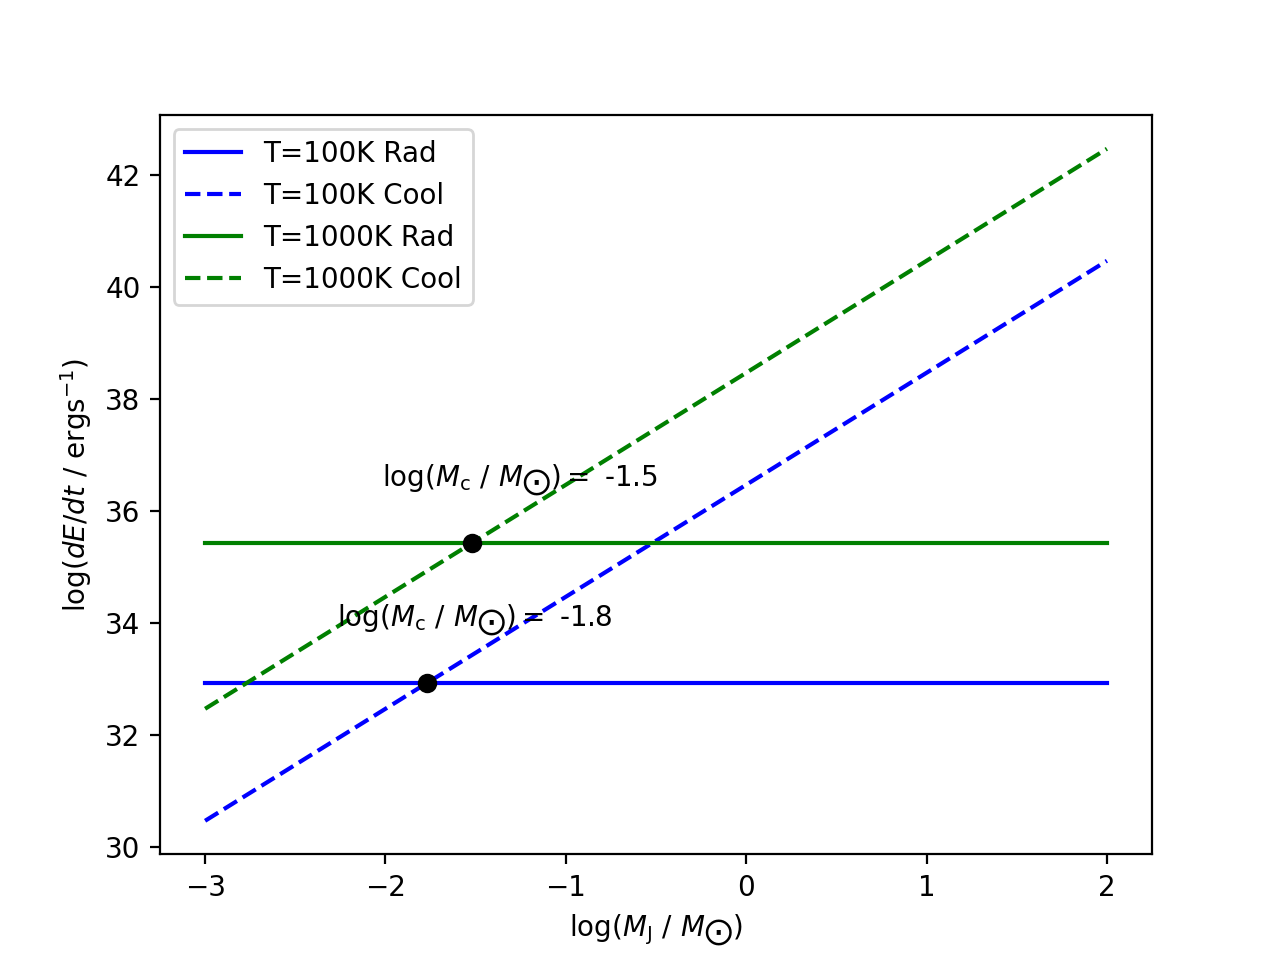
\includegraphics[width=10cm]{frag.png}
    % \caption{The relation}
\end{figure}

\subsection*{(f)}
Fragmentation stops at this point because if the Jeans Mass gets further smaller, 
the rate of radiation will be greater than the rate of cooling. When the rate of radiation 
is greater than the rate of cooling, cooling becomes uneffective and 
heat will be trapped, transforming the process from isothermal to adiabatic and 
increasing the Jeans Mass. With the Jeans Mass increased, the fragmentation stops.

\section*{\textbf{Exercise \uppercase\expandafter{\romannumeral3}.6 Planet formation}}
\subsection*{(a)}
The relative motion between $M$ and $m$ is the radial velocity of $m$ caused by the eccentricity of m-bodies.
The radial velocity of the m-bodies can be estimated as the radial difference at the aphelion and the  perihelion 
divided by one half of the orbital period.
\begin{align*}
    v_r &\sim  \frac{2c}{T/2} = \frac{2ea}{T/2} \\
    \Omega_k &= \frac{2\pi}{T} \\
    v_r &\sim \frac{2ea}{\pi } \Omega_k
\end{align*}
The scale height of the m-bodies is $H \sim ai = ae/2$, so the number density of the m-bodies is:
\begin{align*}
    n \sim \frac{\Sigma_m}{H m}
\end{align*}
Assuming the collision cross section is $\sigma_m = \pi R^2$, the collision time can be written as:
\begin{align*}
    t_\text{coll} = \frac{1}{n\sigma_m \Delta v} \sim \frac{1}{n\sigma_m v_r} = \frac{m}{4\Sigma_m R^2 \Omega_k}
\end{align*}
The mass increasing rate for $M$ is:
\begin{align*}
    \frac{\d M}{\d t} = \frac{m}{t_\text{coll}} = 4 \Sigma_m R^2 \Omega_k
\end{align*}
Therefore, the growth timescale of the M-body is:
\begin{equation*}
    t_\text{growth} = \frac{M}{\d M/\d t} = \frac{\pi}{3} \frac{R \rho_\bullet }{\Sigma_m \Omega_k} \sim \frac{R \rho_\bullet }{\Sigma_m \Omega_k}
\end{equation*}

\subsection*{(b)}
\begin{enumerate}
    \item[] 0.1 au: $t_\text{growth} = 1.77 \times 10^5 \ \text{yrs}$
    \item[] 1 au: $t_\text{growth} = 5.61 \times 10^7 \ \text{yrs}$ 
    \item[] 10 au: $t_\text{growth} = 1.77 \times 10^{10} \ \text{yrs}$ 
\end{enumerate}
\textcolor{red}{The timescales are too long to explain the solar system's planets. As we all know, 
the age of the Sun is about 4.6Gyr and the age of the Earth is about 4.5Gyr. 
The timescale for 10au is larger than the age of the solar system.
For 1au, the timescale is a bit smaller than 1Gyr, but the }

\subsection*{(c)}
If we consider gravitational focusing, then the collision cross section will become:
\begin{align*}
    \sigma_g = \pi R^2 (1+(\frac{v_\text{esc}}{\Delta v})^2) = \pi R^2 (1 + \frac{2GM}{R \Delta v^2}) \sim \pi R^2 (1 + \frac{2GM}{R v_r^2})
\end{align*}
The mass increasing rate for M-body will become:
\begin{align*}
    \frac{\d M}{\d t} &= 4 \Sigma_m R^2 \Omega_k (1 + \frac{2GM}{R v_r^2})
\end{align*}
This is a differential equation for M, and we seperate variables:
\begin{align*}
    \frac{\d M}{1 + \frac{2GM}{R v_r^2}} = 4 \Sigma_m R^2 \Omega_k \d t
\end{align*}
We integrate the above equation and notice that $M(t=0)=0$:
\begin{align*}
    t_\text{growth} = \frac{v_r^2}{8G\Sigma_m R \Omega_k} \ln (1+\frac{2GM}{R v_r^2}) 
\end{align*}
Growth timescales:
\begin{enumerate}
    \item[] 0.1 au: $t_\text{growth} = 3.13 \times 10^3 \ \text{yrs}$
    \item[] 1 au: $t_\text{growth} = 1.38 \times 10^5 \ \text{yrs}$ 
    \item[] 10 au: $t_\text{growth} = 5.59 \times 10^6 \ \text{yrs}$ 
\end{enumerate}

\end{document}
